\section{Date: 2026-08-24}
\noindent \textbf{Series ID: DTBOOXDFBANM} 

\noindent This series is titled Other Business Receivables Owned by Finance Companies, Flow and has a frequency of Monthly. The units are Millions of Dollars, Monthly Rate and the seasonal adjustment is Not Seasonally Adjusted.The observation start date is 1980-07-01 and the observation end date is 2026-05-01.The popularity of this series is 1. \\ 

\noindent \textbf{Series ID: SMS00000000000000022} 

\noindent This series is titled Diffusion Indexes, 3-Month Span: Total Nonfarm and has a frequency of Monthly. The units are Index and the seasonal adjustment is Seasonally Adjusted.The observation start date is 1991-01-01 and the observation end date is 2026-07-01.The popularity of this series is 17. \\ 

\subsection{Raw Regression}
\noindent Regresses the two series against each other directly. A significant result here can come just as easily from both series sharing a long-run trend as from any real relationship.

\begin{center}
\begin{tabular}{lclc}
\toprule
\textbf{Dep. Variable:}            & value\_fred\_SMS00000000000000022 & \textbf{  R-squared:         } &     0.007   \\
\textbf{Model:}                    &                OLS                & \textbf{  Adj. R-squared:    } &     0.004   \\
\textbf{Method:}                   &           Least Squares           & \textbf{  F-statistic:       } &     2.780   \\
\textbf{Date:}                     &          Mon, 24 Aug 2026         & \textbf{  Prob (F-statistic):} &   0.0962    \\
\textbf{Time:}                     &              12:21:23             & \textbf{  Log-Likelihood:    } &   -1980.1   \\
\textbf{No. Observations:}         &                  425              & \textbf{  AIC:               } &     3964.   \\
\textbf{Df Residuals:}             &                  423              & \textbf{  BIC:               } &     3972.   \\
\textbf{Df Model:}                 &                    1              & \textbf{                     } &             \\
\textbf{Covariance Type:}          &             nonrobust             & \textbf{                     } &             \\
\bottomrule
\end{tabular}
\begin{tabular}{lcccccc}
                                   & \textbf{coef} & \textbf{std err} & \textbf{t} & \textbf{P$> |$t$|$} & \textbf{[0.025} & \textbf{0.975]}  \\
\midrule
\textbf{const}                     &      76.2916  &        1.244     &    61.331  &         0.000        &       73.847    &       78.737     \\
\textbf{value\_fred\_DTBOOXDFBANM} &       0.0009  &        0.001     &     1.667  &         0.096        &       -0.000    &        0.002     \\
\bottomrule
\end{tabular}
\begin{tabular}{lclc}
\textbf{Omnibus:}       & 115.402 & \textbf{  Durbin-Watson:     } &    0.217  \\
\textbf{Prob(Omnibus):} &   0.000 & \textbf{  Jarque-Bera (JB):  } &  214.702  \\
\textbf{Skew:}          &  -1.569 & \textbf{  Prob(JB):          } & 2.39e-47  \\
\textbf{Kurtosis:}      &   4.511 & \textbf{  Cond. No.          } & 2.40e+03  \\
\bottomrule
\end{tabular}
%\caption{OLS Regression Results}
\end{center}

Notes: \newline
 [1] Standard Errors assume that the covariance matrix of the errors is correctly specified. \newline
 [2] The condition number is large, 2.4e+03. This might indicate that there are \newline
 strong multicollinearity or other numerical problems.

\begin{figure}
\centering
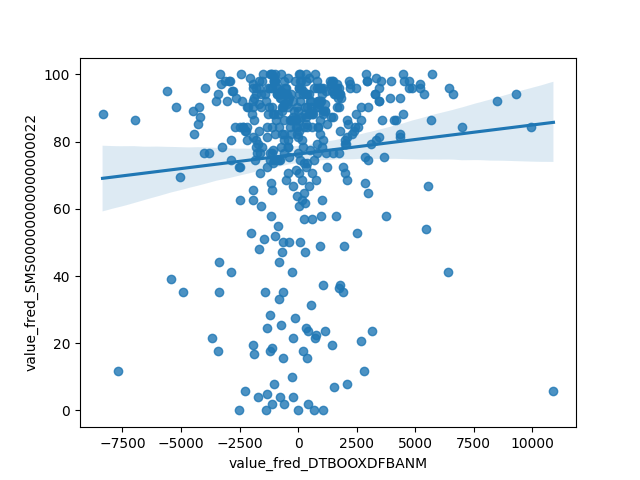
\includegraphics[scale = 0.9]{plots/plot_2026-08-24.png}
\caption{Raw Regression Plot for 2026-08-24}
\end{figure}
\newpage
\subsection{Detrended Regression}
\noindent Regresses the residuals of each series after removing its own linear time trend, so a shared trend can no longer drive the result on its own. A relationship that stays significant here is better evidence of a genuine link between the two series.

\begin{center}
\begin{tabular}{lclc}
\toprule
\textbf{Dep. Variable:}                       & value\_fred\_SMS00000000000000022\_detrended & \textbf{  R-squared:         } &     0.006   \\
\textbf{Model:}                               &                     OLS                      & \textbf{  Adj. R-squared:    } &     0.004   \\
\textbf{Method:}                              &                Least Squares                 & \textbf{  F-statistic:       } &     2.758   \\
\textbf{Date:}                                &               Mon, 24 Aug 2026               & \textbf{  Prob (F-statistic):} &   0.0975    \\
\textbf{Time:}                                &                   12:21:24                   & \textbf{  Log-Likelihood:    } &   -1980.1   \\
\textbf{No. Observations:}                    &                       425                    & \textbf{  AIC:               } &     3964.   \\
\textbf{Df Residuals:}                        &                       423                    & \textbf{  BIC:               } &     3972.   \\
\textbf{Df Model:}                            &                         1                    & \textbf{                     } &             \\
\textbf{Covariance Type:}                     &                  nonrobust                   & \textbf{                     } &             \\
\bottomrule
\end{tabular}
\begin{tabular}{lcccccc}
                                              & \textbf{coef} & \textbf{std err} & \textbf{t} & \textbf{P$> |$t$|$} & \textbf{[0.025} & \textbf{0.975]}  \\
\midrule
\textbf{const}                                &     4.49e-14  &        1.242     &  3.62e-14  &         1.000        &       -2.441    &        2.441     \\
\textbf{value\_fred\_DTBOOXDFBANM\_detrended} &       0.0009  &        0.001     &     1.661  &         0.098        &       -0.000    &        0.002     \\
\bottomrule
\end{tabular}
\begin{tabular}{lclc}
\textbf{Omnibus:}       & 115.439 & \textbf{  Durbin-Watson:     } &    0.217  \\
\textbf{Prob(Omnibus):} &   0.000 & \textbf{  Jarque-Bera (JB):  } &  214.833  \\
\textbf{Skew:}          &  -1.569 & \textbf{  Prob(JB):          } & 2.24e-47  \\
\textbf{Kurtosis:}      &   4.513 & \textbf{  Cond. No.          } & 2.39e+03  \\
\bottomrule
\end{tabular}
%\caption{OLS Regression Results}
\end{center}

Notes: \newline
 [1] Standard Errors assume that the covariance matrix of the errors is correctly specified. \newline
 [2] The condition number is large, 2.39e+03. This might indicate that there are \newline
 strong multicollinearity or other numerical problems.

\begin{figure}
\centering
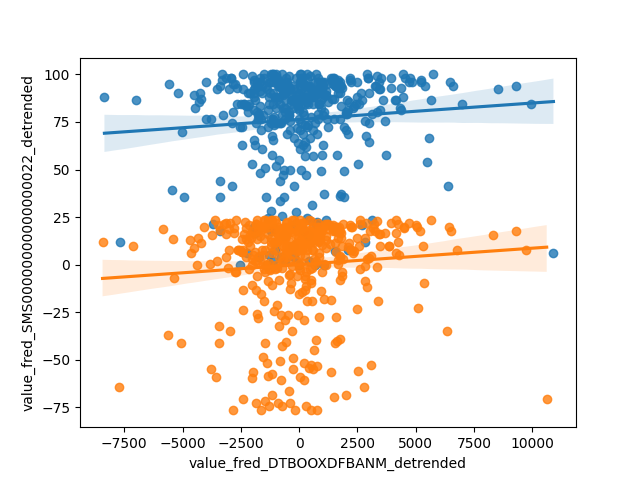
\includegraphics[scale = 0.9]{plots/plot_2026-08-24_detrended.png}
\caption{Detrended Regression Plot for 2026-08-24}
\end{figure}
\newpage
